%==============================================================================
% Chapitre 67 - L'amorce et son inflammation
%==============================================================================

\section{Introduction}

Le départ d'un coup débute par l'action du percuteur sur l'amorce.

Bien que de très petite taille, l'amorce joue un rôle fondamental. Elle
constitue la source initiale d'énergie permettant d'enflammer la charge de
poudre.

Sans son fonctionnement correct, aucun tir n'est possible.

\begin{aretenir}

L'amorce est le premier élément actif du cycle de tir.

\end{aretenir}

\section{Rôle de l'amorce}

L'amorce a pour fonction principale de produire une flamme suffisamment
énergétique pour initier la combustion de la poudre.

Elle constitue une interface entre le mécanisme de percussion et la charge
propulsive.

\section{Principe général}

L'énergie mécanique transmise par le percuteur est transformée en énergie
chimique puis en énergie thermique.

Cette transformation se déroule en quelques fractions de milliseconde.

\begin{figure}[htbp]
\centering

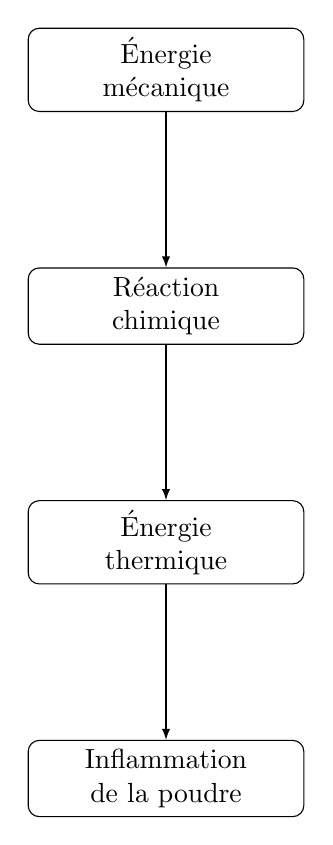
\begin{tikzpicture}[
every node/.style={
draw,
rounded corners,
align=center,
minimum width=3.5cm
}
]

\node (M) at (0,0)
{Énergie\\mécanique};

\node (A) at (0,-3)
{Réaction\\chimique};

\node (T) at (0,-6)
{Énergie\\thermique};

\node (P) at (0,-9)
{Inflammation\\de la poudre};

\draw[-latex] (M) -- (A);
\draw[-latex] (A) -- (T);
\draw[-latex] (T) -- (P);

\end{tikzpicture}

\caption{Transformation de l'énergie lors du fonctionnement de l'amorce.}
\label{fig:chaine_energetique_amorce}

\end{figure}

\section{La percussion}

Lorsque le tireur agit sur la détente, le mécanisme de percussion libère le
percuteur.

Celui-ci frappe la coupelle de l'amorce avec une vitesse élevée.

\section{Déformation de la coupelle}

Sous l'effet du choc, la coupelle métallique se déforme.

Cette déformation provoque l'écrasement de la composition pyrotechnique entre
la coupelle et l'enclume.

\begin{figure}[htbp]
\centering

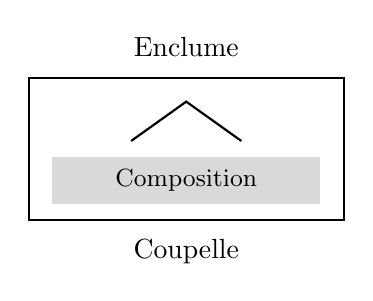
\begin{tikzpicture}[scale=1]

% Coupelle
\draw[thick]
(-2,0)
rectangle
(2,1.8);

% Composition
\fill[gray!30]
(-1.7,0.2)
rectangle
(1.7,0.8);

% Enclume
\draw[thick]
(-0.7,1.0)
--
(0,1.5)
--
(0.7,1.0);

\node at (0,0.5)
{\small Composition};

\node at (0,2.2)
{Enclume};

\node at (0,-0.4)
{Coupelle};

\end{tikzpicture}

\caption{Principe simplifié d'une amorce de type Boxer.}
\label{fig:amorce_boxer_simplifiee}

\end{figure}

\section{Composition pyrotechnique}

La composition d'amorçage contient plusieurs composants chimiques destinés à
réagir rapidement sous l'effet d'un choc mécanique.

Les formulations exactes varient selon les fabricants et les applications.

\section{Réaction initiale}

L'écrasement de la composition provoque une réaction extrêmement rapide.

Cette réaction libère une quantité importante d'énergie dans un volume très
réduit.

\begin{figure}[htbp]
\centering

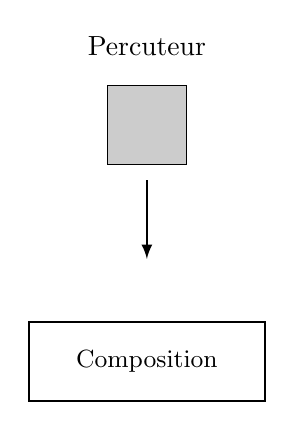
\begin{tikzpicture}

% Percuteur
\draw[fill=gray!40]
(0,3)
rectangle
(1,4);

\node at (0.5,4.5)
{Percuteur};

\draw[-latex,thick]
(0.5,2.8)
--
(0.5,1.8);

% Amorce
\draw[thick]
(-1,0)
rectangle
(2,1);

\node at (0.5,0.5)
{\small Composition};

\end{tikzpicture}

\caption{Écrasement de la composition pyrotechnique sous l'effet du percuteur.}
\label{fig:ecrasement_composition}

\end{figure}

\section{Production de gaz chauds}

La réaction génère des gaz à haute température.

Ces gaz contribuent à l'allumage de la poudre située dans l'étui.

\section{Production de particules incandescentes}

Outre les gaz, l'amorce produit généralement des particules solides portées à
haute température.

Ces particules participent également à l'inflammation de la charge propulsive.

\section{Transmission de la flamme}

Les gaz et particules issus de l'amorce traversent le ou les évents de
l'étui.

Ils atteignent alors la charge de poudre.

\begin{figure}[htbp]
\centering

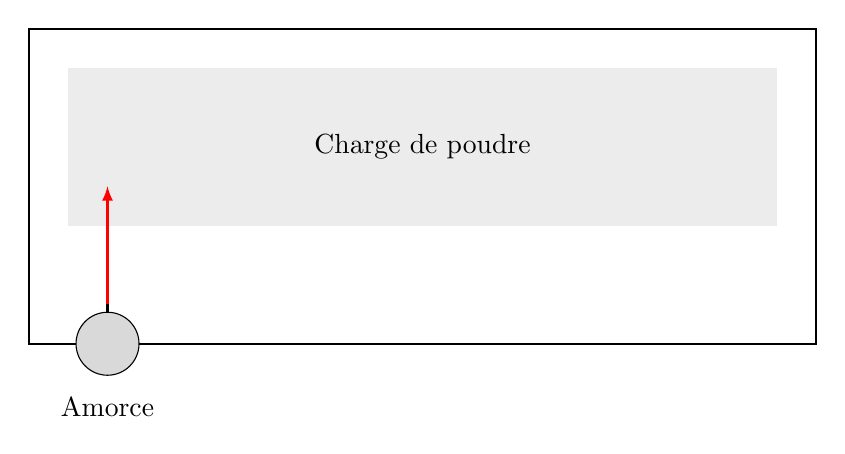
\begin{tikzpicture}

% Étui
\draw[thick]
(0,0)
rectangle
(10,4);

% Amorce
\draw[fill=gray!30]
(1,0)
circle (0.4);

\node at (1,-0.8)
{Amorce};

% Event
\draw[thick]
(1,0.4)
--
(1,1.2);

% Poudre
\fill[gray!15]
(0.5,1.5)
rectangle
(9.5,3.5);

\node at (5,2.5)
{Charge de poudre};

% Flamme
\draw[-latex,red,thick]
(1,0.5)
--
(1,2);

\end{tikzpicture}

\caption{Transmission des produits de réaction de l'amorce vers la poudre.}
\label{fig:transmission_flamme}

\end{figure}

\section{Début de l'inflammation de la poudre}

L'inflammation de la poudre ne se produit pas instantanément dans toute la
cartouche.

Elle débute localement dans les zones atteintes par les produits de
combustion de l'amorce.

\section{Temps caractéristiques}

L'ensemble de ces phénomènes se déroule sur des durées extrêmement courtes.

Les délais observés sont généralement de l'ordre de quelques millisecondes ou
moins.

\begin{figure}[htbp]
\centering

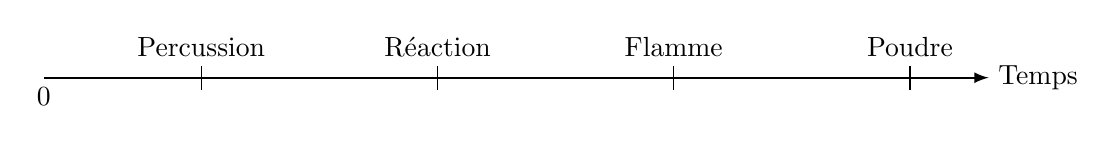
\begin{tikzpicture}

\draw[-latex,thick]
(0,0)
--
(12,0);

\node[below] at (0,0)
{0};

\draw (2,0.15) -- (2,-0.15);
\node[above] at (2,0.15)
{Percussion};

\draw (5,0.15) -- (5,-0.15);
\node[above] at (5,0.15)
{Réaction};

\draw (8,0.15) -- (8,-0.15);
\node[above] at (8,0.15)
{Flamme};

\draw (11,0.15) -- (11,-0.15);
\node[above] at (11,0.15)
{Poudre};

\node[right] at (12,0)
{Temps};

\end{tikzpicture}

\caption{Succession simplifiée des phénomènes liés à l'amorce.}
\label{fig:chronologie_amorcage}

\end{figure}

\section{Ratés de tir}

Il arrive qu'une amorce ne fonctionne pas correctement.

On distingue notamment :

\begin{itemize}
    \item les ratés complets ;
    \item les départs retardés ;
    \item les allumages incomplets.
\end{itemize}

Ces situations peuvent avoir diverses causes mécaniques ou chimiques.

\section{Sécurité}

En présence d'un départ retardé, il convient de conserver l'arme dirigée dans
une direction sûre pendant un certain temps.

Un départ peut en effet se produire après un délai inhabituel.

\section{Influence sur les performances}

La qualité de l'amorçage influence directement :

\begin{itemize}
    \item la régularité des pressions ;
    \item la vitesse initiale ;
    \item la dispersion des résultats ;
    \item la fiabilité du système.
\end{itemize}

\section{Observation expérimentale}

L'étude des amorces peut être réalisée à l'aide de moyens expérimentaux tels
que :

\begin{itemize}
    \item les caméras rapides ;
    \item les capteurs de pression ;
    \item les dispositifs d'acquisition ;
    \item les essais instrumentés.
\end{itemize}

\section{Amorce et simulation}

\begin{simulation}

Dans les modèles simplifiés de balistique intérieure, l'amorce est souvent
représentée comme une source d'énergie initiale.

Les réactions chimiques détaillées sont rarement simulées individuellement.

Le modèle cherche généralement à reproduire correctement le délai d'allumage
et l'initiation de la combustion de la poudre.

\end{simulation}

\begin{figure}[htbp]
\centering

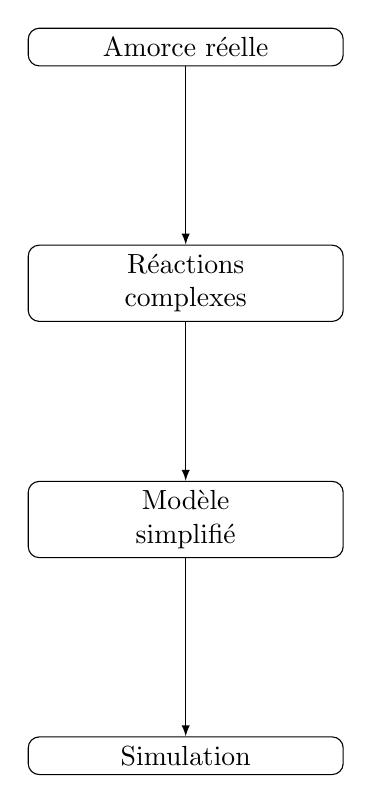
\begin{tikzpicture}[
every node/.style={
draw,
rounded corners,
align=center,
minimum width=4cm
}
]

\node (R) at (0,0)
{Amorce réelle};

\node (C) at (0,-3)
{Réactions\\complexes};

\node (M) at (0,-6)
{Modèle\\simplifié};

\node (S) at (0,-9)
{Simulation};

\draw[-latex] (R) -- (C);
\draw[-latex] (C) -- (M);
\draw[-latex] (M) -- (S);

\end{tikzpicture}

\caption{Principe de simplification utilisé dans les modèles de simulation.}
\label{fig:simulation_amorce}

\end{figure}

\section{Vers la combustion de la poudre}

L'action de l'amorce ne constitue que la première étape du cycle de tir.

La phase suivante correspond à la combustion de la charge propulsive, qui
produira la majeure partie des gaz responsables de l'accélération du
projectile.

\section{À retenir}

\begin{aretenir}

\begin{itemize}
    \item L'amorce transforme l'énergie mécanique du percuteur en énergie thermique.
    \item La composition pyrotechnique réagit sous l'effet du choc.
    \item L'amorce produit des gaz chauds et des particules incandescentes.
    \item Ces produits enflamment la poudre.
    \item La qualité de l'amorçage influence les performances du tir.
\end{itemize}

\end{aretenir}
